\documentclass[11pt,a4paper,landscape]{article}
\usepackage[utf8]{inputenc}
\usepackage[english]{babel}
\usepackage[left=2cm,right=2cm,top=2cm,bottom=2cm]{geometry}
\usepackage{fancyhdr}
\usepackage{multicol}
\usepackage{graphicx}
\usepackage{siunitx}
\usepackage{amsmath}
\usepackage{amssymb}
\usepackage{wrapfig}
\usepackage{float}


\author{Himanshu Mittal}
\title{Tangent and Normal}

\renewcommand{\labelenumi}{\theenumi}

\everymath{\displaystyle}
\pagestyle{fancy}
\fancyhf{}
\graphicspath{{./images/}}

\renewcommand{\headrulewidth}{0pt}
\renewcommand{\footrulewidth}{2pt}
\setlength\parindent{0pt}
\lfoot{\bfseries Himanshu Mittal : mittal01091997@gmail.com} 

\begin{document}
\begin{multicols*}{2}
\textbf{\Huge{Tanget and Normal}}
\section{Tangent And Normal}
	\subsection{Introuction}
	Let equation of a curve be $y=f(x)$.\\[1mm]
	And its first derevative be $\frac{dy}{dx}=\frac{d}{dx}(f(x))$.
	\begin{figure}[H]
		\centering
		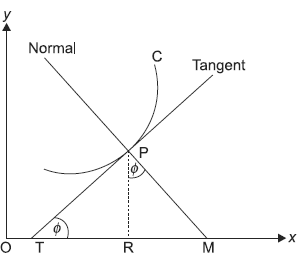
\includegraphics[width=6cm]{P1}
		\caption{Tangent and Normal}
	\end{figure}

	\textbf{Slope of Tangent:}
	\begin{itemize}
	\item at point P: $\frac{dy}{dx}$
	\item parallel to $x$-axis: $\frac{dy}{dx}(x_1,y_1)=0$
	\item parallel to $y$-axis: $\frac{dy}{dx}(x_1,y_1)=\infty$
	\end{itemize}

	\textbf{Slope of Normal:} at point P = $\frac{-1}{\frac{dy}{dx}}$ or $\frac{-dx}{dy}$
	\subsection{Equations}
	$y-y_1=m(x-x_1)$ where $(x_1,y_1)$ is the point of tangent and normal.\\[2mm]
	\textbf{For Tangent:} $y-y_1=\left(\frac{dy}{dx}\right)_P(x-x_1)$\\[3mm]
	\textbf{For Normal:} $y-y_1=\frac{-1}{\left(\frac{dy}{dx}\right)_P}(x-x_1)$
\section{Angle between two curves}
	\subsection{Angle of Intersection}
	let $C_1=y=f(x)$ and $C_2=y=(x)$.
	\begin{figure}[H]
		\centering
		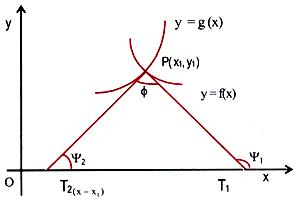
\includegraphics[width=7cm]{P2}
		\caption{Angle between Curves}
	\end{figure}
	$PT_1$ = tangent to $C_1$ and $PT_2$ = tangent to $C_2$.\\
	Then,\\
	$m_1=\tan{\psi_1}$ = slope of tangent of $y=f(x)$ at $P=\left(\frac{dy}{dx}\right)_{C_1}$\\[2mm]
	$m_2=\tan{\psi_2}$ = slope of tangent of $y=g(x)$ at $P=\left(\frac{dy}{dx}\right)_{C_2}$\\[2mm]
	$\phi=\psi_1-\psi_2$\\
	or, $\tan{\phi}=\frac{\tan{\psi_1}-\tan{\psi_2}}{1-\tan{\psi_1}\tan{\psi_2}}$\\[3mm]
	or, $\tan{\phi}=\frac{\left(\frac{dy}{dx}\right)_{C_1}-\left(\frac{dy}{dx}\right)_{C_2}}{1+\left(\frac{dy}{dx}\right)_{C_1}\left(\frac{dy}{dx}\right)_{C_2}}$\\[3mm]
	\textbf{Note:} The other angle between tangents = $\ang{180}-\theta$
	\subsection{Orthogonal Curves}
	If angle of Intersection of two curves is a right angle, the curves are orthogonal curves. \textbf{i.e.} $\phi=\frac{\pi}{2}$\\[2mm]
	$\therefore m_1m_2 = -1 \Rightarrow \left(\frac{dy}{dx}\right)_{C_1} \cdot \left(\frac{dy}{dx}\right)_{C_2} = -1$
\section{Subtangent and Subnormal}
	Let $y=f(x)$ be a curve. Let $\frac{dy}{dx}=f'(x)$ be the slope.
	\begin{figure}[H]
		\centering
		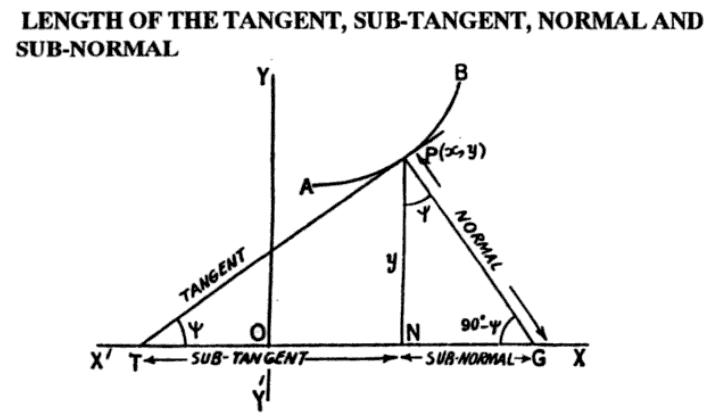
\includegraphics[width=7cm]{P3}
		\caption{Various lengths}
	\end{figure}	
	Let the tangent and normal touch $x$-axis at point T and N respectively. If G is a perpendicular to P, then:
	\begin{itemize}
	\item Length of subtangent (TG) = $|y\cot\psi| = \left|\frac{y}{\frac{dy}{dx}}\right|$
	\item Length of subnormal (NG) = $|y\tan\psi| = \left|y\frac{dy}{dx}\right|$
	\item If PT makes an angle $\psi$ with $x$-axis, then $\tan\psi = \frac{dy}{dx}$
	\item Length of tangent (PT) = $|y\,cosec\,\psi|$\\[2mm]
	$= |y\sqrt{1+\cot^2{\psi}}|$\\[3mm]
	$= \left|y\frac{\sqrt{1+\left(\frac{dy}{dx}\right)^2}}{\frac{dy}{dx}}\right|$
	\item Length of Normal (PN) = $|y\sec{\psi}|$\\[2mm]
	$= |y\sqrt{1+\tan^2{\psi}}|$\\[3mm]
	$= \left|y\sqrt{1+\left(\frac{dy}{dx}\right)^2}\right|$
	\end{itemize}
\end{multicols*}
\end{document}
